\chapter{Pojem fyzikální model a~jeho vlastnosti}

Fyzikálním modelem řídicího systému chápu seznam pravidel, či vzorců, dle kterého lze určit polohu stroje (jednotlivých os) v~kterémkoliv okamžiku v~čase $t$. Tudíž mou snahou je vyjádřit všechny potřebné veličiny  v~závisloti na čase $t$. G-kód definuje dva druhy pohybu\cite{gcode} -- pohyb přímočarý (po úsečce) a~pohyb po kruhovém oblouku -- pro každý je nutné vytvořit samostatný model.

Vstupem do fyzikálního modelu jsou limitující faktory a~jednotlivé úseky (dílčí pohyby) zadané programem v~G-kódu, po kterých se má stroj pohybovat. Každý dílčí pohyb se skládá ze tří částí -- zrychlení z~počáteční rychlosti~$v_0$ na zadanou cílovou rychlost~$V$, pohybu rovnoměrného přímočarého rychlostí~$V$ a~zpomalení na danou brzdnou rychlost~$v_b$. Ve~speciálních případech může být vynechán rovnoměrný přímočarý pohyb, nebo rychlost $v_0$ (potažmo $v_b$) je rovna rychlosti $V$ -- tedy nedojde k~zrychlování, respektive zpomalování.

Z pohledu fyzikálního modelu je nejdůležitější se zaměřit na zrychlování, resp. zpomalování, jelikož na pohybu rovnoměrném přímočarém není co řešit.

	\section{Vlastnosti ideálního fyzikálního modelu}\label{kap:vlastnostimodelu}
	Ideální fyzikální model by měl dosáhnout co nejplynulejšího a~nejrychlejšího pohybu (v~zájmu zrychlení obrábění). Zároveň však musí respektovat mechanické limity stroje. Jedním ze způsobů, jak toho docílit, je vhodně nastavit akcelerační křivky (průběh rychlosti v~závisosti na čase) a~tím omezit rázy. Rázem chápu prudkou změnu působícího zrychlení a~tudíž i působící síly. Je tedy nutno určit, jak tyto mechanické limity definovat, což provádím v~kapitole \ref{kap:limitujicifaktory}.
	
	\section{Fyzikální veličina ryv}
	Běžně se pro charakteristiku pohybu používá rychlost a~zrychlení. Pro popsání pohybu z~hlediska dynamiky je však vhodné uvažovat ještě třetí veličinu -- ryv (anglicky jerk), značený $j$\cite{wiki:ryv}. Ryv je definován následovně\cite{wiki:ryv}:
	\begin{equation}
		\vec{j}=\frac{\dif \vec{a}}{\dif t}=\frac{\dif^2 \vec{v}}{\dif t^2}=\frac{\dif^3 \vec{d}}{\dif t^3},
	\end{equation}
	kde $\vec{a}$ je zrychlení pohybu, $\vec{v}$ je rychlost pohybu a~$\vec{d}$ je poloha tělesa v~prostoru. Jednotkou ryvu je $1~$m$\cdot$s$^{-3}$. Ryv popisuje změnu zrychlení v~čase. Název ryv byl odvozen od českého slova \uv{poryv}\cite{wiki:ryvcz} (anglického jerk -- cukat\cite{wiki:ryv}).
	
	\section{Akcelerační křivky}\label{kap:akckriv}
	Akcelerační křivkou se běžně označuje graf závislosti rychlosti pohybu na čase. Na grafu \ref{graf:konstant} je znázorněna akcelerační křivka běžně používaného modelu zrychlení na hobby CNC strojích -- za použití konstantního zrychlení.
	
	\begin{figure}[h]
		\centering
		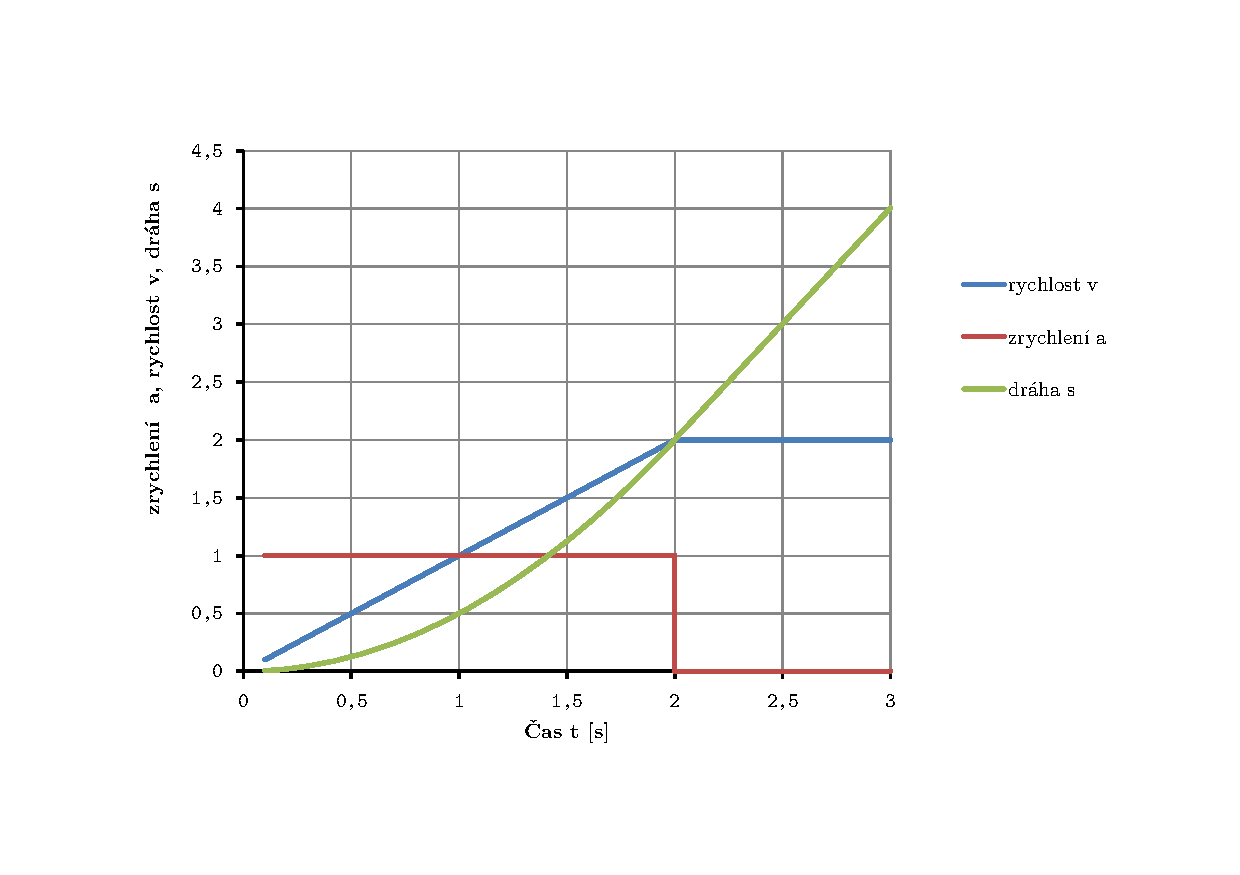
\includegraphics[width=0.9\textwidth]{img/graf_konstant.pdf}
		\caption{Akcelerační křivka konstantního zrychlení.} \label{graf:konstant}
	\end{figure}
	
	Sklon křivky rychlosti (tedy derivace rychlosti) ukazuje aktuální zrychlení. Z~Newtonova zákona síly vyplývá, že působící síla je přímo úměrná zrychlení. Pokud tedy zrychlení ustane (na grafu \ref{graf:konstant} v~čase $t=2~s$), prudce ustane i působící síla a~nastane ráz -- prudké odlehčení zátěže ze~stroje. Obdobná situace nastává i při nástupu zrychlení (zde v~čase $t=0~s$). Tyto jevy nastávají při ostrém zlomu na grafu rychlosti v~závislosti na čase.
	 
	Pokud se na situaci podíváme z~pohledu ryvu, tak vidíme, že zrychlení je nespojitou funkcí času, tudíž jeho derivace v~bodech nespojitosti není definována. To je však pouze teoretická situace. Ve skutečnosti je zrychlení stále spojitou funkcí, ovšem s~velmi strmými přechody. Ryv zde tedy dosahuje obrovských hodnot (dokonce můžeme mluvit až o $j\rightarrow\infty$). Velikost ryvu charakterizuje tyto prudké změny zrychlení, a~tedy i změnu zátěže.
	
	Z výše uvedeného lze usoudit, že pro nejplynulejší pohyb je důležité, aby na grafu rychlosti v~závislosti na čase nedocházelo ke~zlomům. Tehdy bude docházet k~postupnému nárůstu a~úbytku zátěže na stroj. Takovýmto grafem rychlosti je tzv. S-křivka. Tato křivka je na počátku tečná k~ose x a~na svém konci tečná ke~konstantní funkci
	\begin{equation}
		v(t) = V,
	\end{equation}
	kde $V$ je rychlost, které je třeba dosáhnout. Mnou sestrojená S-křivka je ukázána na grafu \ref{graf:linprubeh1} v~kapitole \ref{kap:linrozbrzd}.
	
	Jako vhodná S-křivka se ukazuje kosinusoida
	\begin{equation}
		y=1-\cos x,
	\end{equation}
	která splňuje tečnost k~funkcím $y=0$ a~$y=V$. Kosinusoida není jediná S-křivka. Obdobně můžou sloužit i některé polynomy. Pro mé účely je však kosinusoida výhodná -- je matematicky snadno definovatelná, na celém svém průběhu je \uv{hladká} a symetrická; také její derivace libovolného stupně a integrály libovoného stupně jsou definovány.
	
	Derivací této kosinusoidy je funkce
	\begin{equation}
		y' = \sin x.
	\end{equation}
	Zrychlení pro docílení S-křivky ve tvaru kosinusoidy tedy musí mít sinusový průběh.
	
	Je však také nutné omezit také strmost S-křivky -- pokud by byla příliš strmá, lze ji považovat za podobnou s~přímkou a~její efekt by byl zanedbatelný. K tomuto omezení slouží právě ryv, který omezí strmost zrychlení, čímž omezí i strmost křivky rychlosti.
	
	\section{Postulát pohybu}\label{kap:postulat}
	
	Na základě zkušeností a~úvahy v předcházející části \ref{kap:akckriv} jsem si pro odvození fyzikálního modelu pro můj řídicí systém stanovil následující postulát:
	
	\uv{Pro ideální pohyb bez rázů musí mít zrychlení plynulý nástup a postupný pokles (v~mém případě volím sinusový průběh). Průběh zrychlení je třeba limitovat jak amplitudou zrychlení, tak i maximálním přípustným ryvem.}


\chapter{Odvození fyzikálního modelu}

	V následujícím odvození fyzikálního modelu pro můj systém vycházím z~mého postulátu (kapitola \ref{kap:postulat}). Pro přehlednost jsem si zavedl následující konvenci: okamžitý stav veličin značím malým příslušným písmenem (např. okamžité zrychlení $a$), maximální (omezující a~obvykle vstupní) hodnoty označuji příslušným velkým písmenem (např. maximální amplituda zrychlení $A$).

	\section{Limitující faktory pohybu}\label{kap:limitujicifaktory}
	
	Jak jsem zmínil v části \ref{kap:vlastnostimodelu}, limitujícím faktorem dynamiky pohybu je kvalita (tuhost) mechanické konstrukce stroje. Většina systémů používá omezení maximálního zrychlení a~maximální rychlosti. Do mého systému jsem přidal ještě omezení maximálního ryvu.
	
	Můj systém používá sinusový průběh zrychlení, tudíž limituji amplitudu $A$ tohoto zrychlení a~špičkovou hodnotu ryvu $J$. U~ryvu $J$ se nesnažím docílit jeho přesného průběhu. 
	
	Narozdíl od běžných systémů jsem se rozhodl implementovat veškerá omezení pro celý stroj, nikoliv pro jednotlivé jeho osy. Jednak se v~praxi u hobby strojů minimálně limity pro osy x a~y nastavují zpravidla stejně, také se jedná o zjednodušení a~také jde o jisté přiblížení k~ideálnímu stavu (stroj by se ve směru všech os měl pohybovat stejně).
	
	\section{Pohyb po úsečce}\label{kap:pohybpousecce}
	Pohyb po úsečce je nejjednodušším možným pohybem na stroji.	Z hlediska fyzikálního modelu se na každou část pohybu (zrychlování, pohyb rovnoměrný přímočarý a~zpomalování) dívám jako na samostanou, tzn. každá začíná v čase $t=0$. Pohyb rovnoměrný přímočarý není třeba popisovat, v následující sekci se proto zaměřím pouze na rozjezd a~brzdění. V~první části~(\ref{kap:linrozbrzd}) odvozuji základní vztahy pro tento pohyb s~omezením maximálního zrychlení. V~druhé části (\ref{kap:linryv}) tyto vztahy rozšiřuji o~omezení maximálního ryvu.
	
		\subsection{Rozjezd a~brzdění}\label{kap:linrozbrzd}
		
		Rozjezd a~brzdění jsou z~fyzikálního pohledu naprosto shodné pohyby lišící se pouze směrem zrychlení. Lze na ně tedy uplatnit stejné vztahy.
		
		Dle postulátu musí mít zrychlení pro tento pohyb sinusový průběh, resp. pro rozjezd je třeba kladná půlvlna, pro zpomalení naopak záporná půlvlna. Pokud označím celkovou dobu trvání tohoto rozjezdu, resp. zpomalení, $T$ a~maximální dosažené zrychlení $A$, dostanu následující vztah pro okamžité zrychlení $a$ v~závislosti na čase $t$.
		\begin{equation}
			a=A \sin\frac{\pi t}{T}\label{rov:1}
		\end{equation}
		Integrováním tohoto výrazu pro zrychlení dostanu vztah pro okamžitou rychlost $v$ v závislosti na čase $t$:
		\begin{equation}
			v=\int a(t) \dif t = -\frac{AT}{\pi}\cos  \frac{\pi t}{T} + c
		\end{equation}
		Nyní je však třeba dopočítat konstantu $c$ (v čase $t=0$ je rychlost $v=0$) a~vzorec doplnit o~počáteční rychlost $v_0$:
		\begin{eqnarray}
			\text{Pro } t = 0 \text{ platí } v = 0 \implies -\frac{AT}{\pi} + c = 0  \nonumber \\
			c = \frac{AT}{\pi} \nonumber \\
			v = \frac{AT}{\pi} \left(1 - \cos \frac{\pi t}{T} \right) + v_0	 \label{rov:linrych}
		\end{eqnarray}
		Zde stojí za povšimnutí, že pokud dosadíme zápornou amplitudu zrychlení $A$ a~místo počáteční rychlosti $v_0$ dosadíme brzdnou rychlost $v_b$, získáme platný vzorec pro zpomalený pohyb. Pro přehlednost jej však můžeme zapsat i následovně (s~kladnou amplitudou):
		\begin{equation}
			v = v_b - \frac{AT}{\pi} \left(1 - \cos \frac{\pi t}{T} \right)
		\end{equation}
		
		Tento získaný vztah pro rychlost (\ref{rov:linrych}) můžeme opět zintegrovat a~získat tak vztah pro okamžitou dráhu pohybu $s$ v~závisloti na čase $t$, což je zároveň vzdálenost uražená od počátku pohybu.
		\begin{eqnarray}
			s=\int v(t) \dif t = \frac{AT}{\pi}t - \frac{AT^2\sin \frac{\pi t}{T}}{\pi^2} + c \nonumber \\
			s = \frac{AT}{\pi^2}\left( \pi t - T \sin \frac{\pi t}{T}\right) \label{rov:lindraha}
		\end{eqnarray}
		
		Dosazením $t=T$ do odvozeného vztahu  pro okamžitou rychlost (\ref{rov:linrych}), dostanu vztah pro maximální dosažitelnou rychlost $V$ za čas $T$ při amplitudě zrychlení $A$ (\ref{rov:linv}), resp. celkovou dobu pohybu $T$ při zadaném zrychlení $A$ (\ref{rov:lincas}), resp. vztah pro potřebné zrychlení ke~změně rychlosti z~$v_0$ na $V$ za čas $T$ (\ref{rov:linzrych}).
		\begin{equation}
			\label{rov:linv}
			V=\frac{2AT}{\pi} + v_0
		\end{equation}
		\begin{equation}
			\label{rov:lincas}
			T=\frac{\pi \left(V - v_0\right)}{2A}
		\end{equation}
		\begin{equation}
			\label{rov:linzrych}
			A=\frac{\pi \left(V - v_0\right)}{2T}
		\end{equation}
		Obdobně jako v předchozím případě lze za $v_0$ dosadit $v_b$ a~získat tak vztahy pro zpomalování.
		
		Stejným dosazením ($t=T$) lze získat i vztah pro celkovou dráhu pohybu pro zrychlování $S$ (\ref{rov:lindrah}), resp. brzdnou dráhu $S_b$ (\ref{rov:lindrahb}):
		\begin{equation}
			\label{rov:lindrah}
			S = \frac{AT^2}{\pi} + v_0 T
		\end{equation}
		\begin{equation}
		\label{rov:lindrahb}
			S_b = VT -\frac{AT^2}{\pi}
		\end{equation}
		
		Z výše uvedených vztahů můžu sestavit vztah pro celkovou dráhu $S$ pohybu po~přímce složeného z~rozjezdu a~zpomalení -- bez rovnoměrného přímočarého pohybu rychlostí $V$:
		\begin{eqnarray}
			S=\frac{AT^2}{\pi} + v_0 T + V T_b -\frac{AT_b^2}{\pi} \nonumber \\
			S=\frac{\pi V\left(V-v_0\right)}{2A}+\frac{\pi \left(V-v_0\right)^2}{4A}+\frac{\pi V\left(V-v_b\right)}{2A}-\frac{\pi \left(V-v_b\right)^2}{4A}
		\end{eqnarray}
		Z tohoto vztahu mohu vyjádřit rychlost $V$, což je vhodné pro nalezení maximální rychlosti, které lze dosáhnout na úsečce o délce $S$ za omezení maximální amplitudou zrychlení $A$:
		\begin{equation}
			V=\frac{\sqrt{4AS+\pi\left(v_0^2-v_b^2\right)}}{2\pi}
		\end{equation}
		Tento vztah lze v praxi použít k~nalezení nové maximální rychlosti, pokud požadované rychlosti nelze na daném úseku dosáhnout.
		
		Na grafech \ref{graf:linprubeh1} a~\ref{graf:linprubeh2} je zobrazen průběh jednotlivých veličin v~závisloti na čase pro výše odvozené vztahy.
		
		\begin{figure}[h]
			\centering
			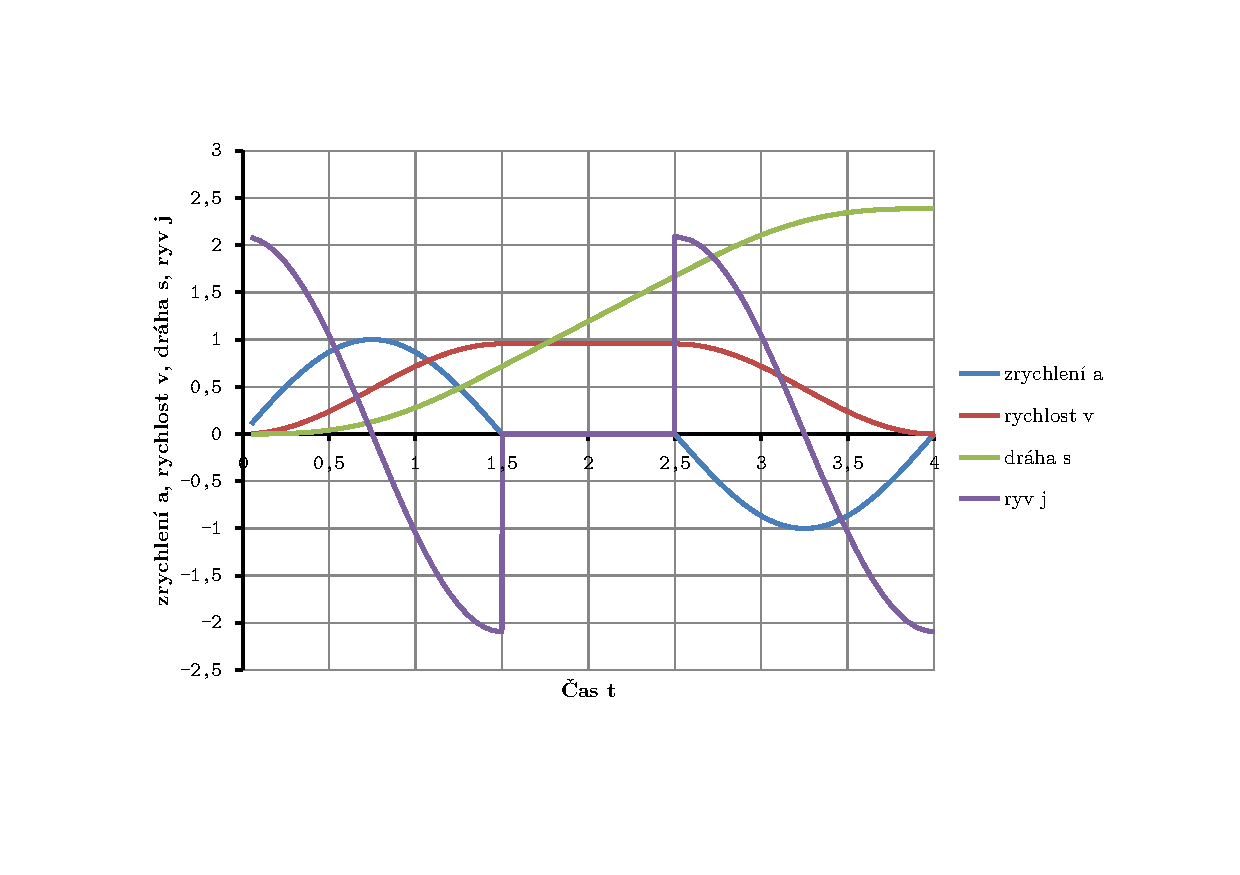
\includegraphics[width=0.9\textwidth]{img/graf_primka1.pdf}
			\caption{Graf znázorňující průběh jednotlivých veličin při použití sinusového zrychlení. Je složen z 1,5 sekundového rozjezdu z rychlosti $v_0=0$; 2 sekundového pohybu přímočarého a~1,5 sekundového brzdění na nulovou rychlost.}\label{graf:linprubeh1}	
		\end{figure}
		
		\begin{figure}[h]
			\centering
			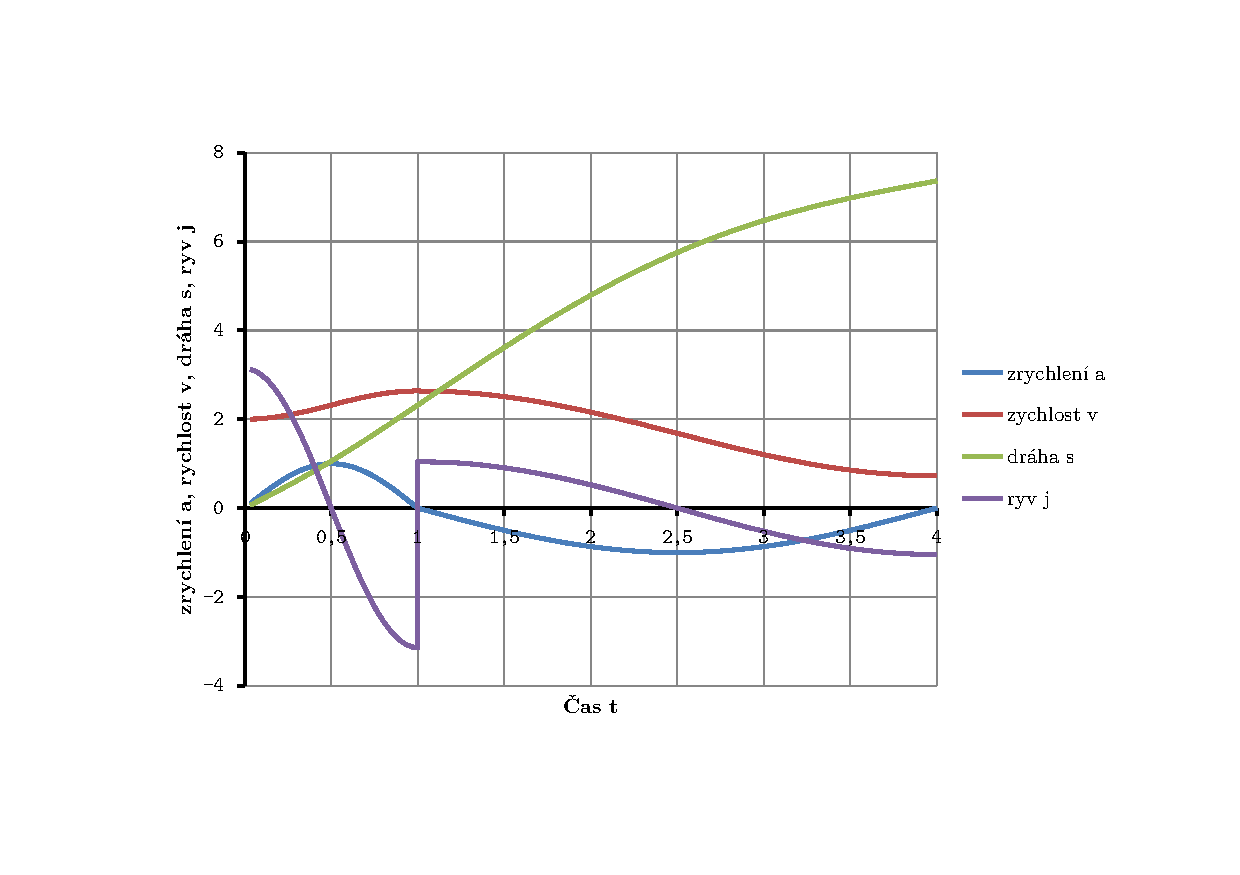
\includegraphics[width=0.9\textwidth]{img/graf_primka2.pdf}
			\caption{Graf znázorňující průběh jednotlivých veličin při použití sinového zrychlení. Je složen ze sekundového rozjezdu z~rychlost $v_0=1$ a~2 sekundového brzdění na brzdnou rychlost $v_b$} \label{graf:linprubeh2}
		\end{figure}
		
		\subsection{Omezení maximálního ryvu}\label{kap:linryv}
		
		Zrychlení není dle postulátu (kapitola \ref{kap:postulat}) jediný omezující faktor. Pro ideální pohyb by měl být omezen i ryv. Ryv ve své aplikaci omezuji pouze jeho špičkovou hodnotou $J$, nikoliv jeho přesně daným průběhem.
		
		Jelikož ryv je definován následovně\cite{wiki:ryv}:
		\begin{equation}
			j=\frac{\dif a}{\dif t},
		\end{equation}
		lze jeho závislost na čase $t$ pro tento konkrétní příklad napsat následovně:
		\begin{equation}
			\label{rov:linryv}
			j=\frac{A \pi}{T} \cos \frac{\pi t}{T}
		\end{equation}
		Průběh ryvu je znázorněn na grafech \ref{graf:linprubeh1} a~\ref{graf:linprubeh2}.
		
		Maximum výrazu pro ryv (\ref{rov:linryv}) je v~čase $t=0$, resp. $t=T$ (zajímá nás i maximální výchylka ryvu do záporných hodnot). Maximální hodnora ryvu $J$ je tedy potom rovna:
		\begin{equation}
			J=\frac{\pi A}{T}
		\end{equation}
		Vyjádřením $A$ z tohoto vztahu a~jeho dosazením do vztahu pro dobu trvání pohybu $T$ (\ref{rov:lincas}) získám omezení pohybu ryvem:
		\begin{equation}
			\label{rov:linTJ}
			T=\frac{\pi}{2}\sqrt{\frac{2\left(V-v_o\right)}{J}}
		\end{equation}
		Zde si je nutno povšimnout, že v tomto vztahu nevystupuje maximální zrychlení $A$, tudíž tento výpočet jím není omezen. Při výpočtu je tedy nutné prvně zkusit spočítat dobu trvání pohybu~$T$ za omezení ryvu a~na základě ní dopočítat maximální zrychlení $A$. Pokud vyjde hodnota $A$ větší než zadaná, je výpočet nutno provést znovu, tentokrát s použitím vztahu \ref{rov:lincas} a~výpočet místo ryvu limitovat zrychlením.
		
		Stejně jako v případě omezení pohybu zrychlením, i zde lze sestavit vztah pro celkovou dráhu pohybu složeného z~rozjezdu a~zpomalení:
		\begin{equation}
				S=\frac{\pi}{2\sqrt{2}} \left(v_b\sqrt{\frac{V-v_b}{J}}-v_0\sqrt{\frac{V-v_0}{J}}+V\left(\sqrt{\frac{V-v_b}{J}}+3\sqrt{\frac{V-v_0}{J}}\right)\right)
		\end{equation} 
		Z této rovnice však nelze získat obecné vyjádření maximální rychlosti $V$, jelikož se jedná o~iracionální rovnici (postupným umocňováním získáme polynom 8. stupně). Je třeba ji řešit numericky.
		
		V prvních verzích řídicího systému jsem tento vztah k~nalezení nové rychlosti používal a~řešil jsem jej Newtonovou metodou, avšak v~poslední verzi jsem jej nahradil hledáním nové rychlosti pomocí bisekce bez použití tohoto vztahu (viz~\ref{kap:rychlost}). U tohoto vztahu je nutné vytvořit jeho několik variant (kombinace rozjezd omezen ryvem, zpomalování zrychlením apod.), aby dával korektní výsledky. Jeho výpočetní náročnost je zhruba totožná s~bisekcí (pokud nejsou rozdíly rychlostí přiliš velké, což v praxi nenastává). Bisekce je dle mě však také elegantnější řešení, které se v~kódu lépe čte. Proto jsem se k~ní nakonec přiklonil.
	
	\section{Pohyb po~kruhovém oblouku}
	
	Pohyb pro kruhovém oblouku je z~hlediska dynamiky na první pohled podobný úsečce. Je zde však nutné uvažovat i~vznikající dostředivé zrychlení, které způsobuje změnu směru pohybu. Zadané omezení špičkového zrychlení tedy neomezuje tečné zrychlení ve~směru pohybu, nýbrž velikost jeho vektorového součtu se~vznikajícím dostředivým zrychlením.
	
	Stejně jako v~kapitole \nameref{kap:pohybpousecce} (\ref{kap:linrozbrzd}) i zde se výsledný pohyb skládá ze tří částí. Jelikož je však rozjezd a~zpomalování totožné (liší se pouze směrem zrychlení) a~pohyb konstantní rychlostí triviální, zaměřím se v této sekci pouze na rozjezd.
	
	Pro zachování souladu s~dříve odvozenými vztahy, kde $A$ reprezentuje zadané omezení zrychlení a~současně reprezentuje maximální velikost tečného zrychlení, budu i nadále označovat maximální velikost tečného zrychlení $A$. Avšak jako omezující faktor zde budu používat velikost celkového zrychlení $A_k$. $A_k$ je tedy vstupním parametrem a~zrychlení $A$ závisí na charakteristice pohybu.  Mým cílem je proto ze zadaných omezení $J$ a~$A_k$ dopočítat hodnoty $T$ a~$A$. Není třeba se zajímat o uraženou dráhu, jelikož tento vztah je po~dosazení přislušných hodnot $A$ a~$T$ stejný jako u~úsečky (vztah \ref{rov:lindrah}).
	
	Jak jsem již zmínil, celkové zrychlení je rovno vektorovému součtu tečného a~dostředivého zrychlení. Jelikož se jedná o pohyb po~kružnici, jsou tato zrychlení na sebe navzájem kolmá, a~proto platí:
	\begin{equation}
		\label{rov:vektrzrych}
		\vec{a_k} = \vec{a}+\vec{a_d}\implies \abs{a_k}=\sqrt{ \abs{a}^2+ \abs{a_d}^2}
	\end{equation}
	
	Dostředivé zrychlení pro pohyb na kružnici o poloměru r je rovno
	\begin{equation}
		a_d = \frac{v^2}{r},
	\end{equation}
	a proto po~dosazení vztahů \ref{rov:1} a~\ref{rov:linrych} do vztahu \ref{rov:vektrzrych} dostanu vyjádření okamžité velikosti zrychlení $a_k$ v závislosti na čase $t$:
	\begin{equation}
		\label{rov:oblzrych}
		a_k=\sqrt{\frac{A^4 T^4 \left(\cos \frac{\pi  t}{T}-1\right)^4}{\pi ^4
		   r^2}+A^2 \sin ^2\frac{\pi  t}{T}}
	\end{equation}
	Derivací tohoto výrazu podle času dostanu vztah pro okamžitý ryv v závisloti na čase $t$:
	\begin{equation}
		\label{rov:oblryv}
		j=\frac{\dif a_k}{\dif t}=\frac{32A^4T^4 \sin^6 \frac{\pi t}{2T}\sin\frac{\pi t}{T}+A^2\pi^4r^2\sin\frac{2\pi t}{T}}{2\pi r^2T\sqrt{\frac{A^4T^4(\cos \frac{\pi t}{T}-1)^4}{r^2}+A^2\pi^4\sin^2\frac{\pi t}{T}}}
	\end{equation}
	
	Pro další pokračování je nutno u těchto vztahů (\ref{rov:oblzrych} a~\ref{rov:vektrzrych}) nalézt jejich maxima. Porovnáním jejich derivací s~nulou jsem získal složité rovnice, které jsou řešitelné pouze numericky. Tomuto řešení jsem se chtěl vyhnout, a~proto jsem začal zkoumat průběhy pro různé kombinace $A$ a~$T$.
	
	Jak lze vidět na grafech \ref{graf:oblprubeh1} a~\ref{graf:oblprubeh2}, mohou nastat dvě situace -- maximum zrychlení se nachází v~čase $t=T$, nebo přibližně v~čase $t=\frac{T}{2}$. Oběma případům se věnuji v~následujících sekcích \ref{kap:maxT} a~\ref{kap:maxT2}.
	
	\begin{figure}[H]
		\centering
		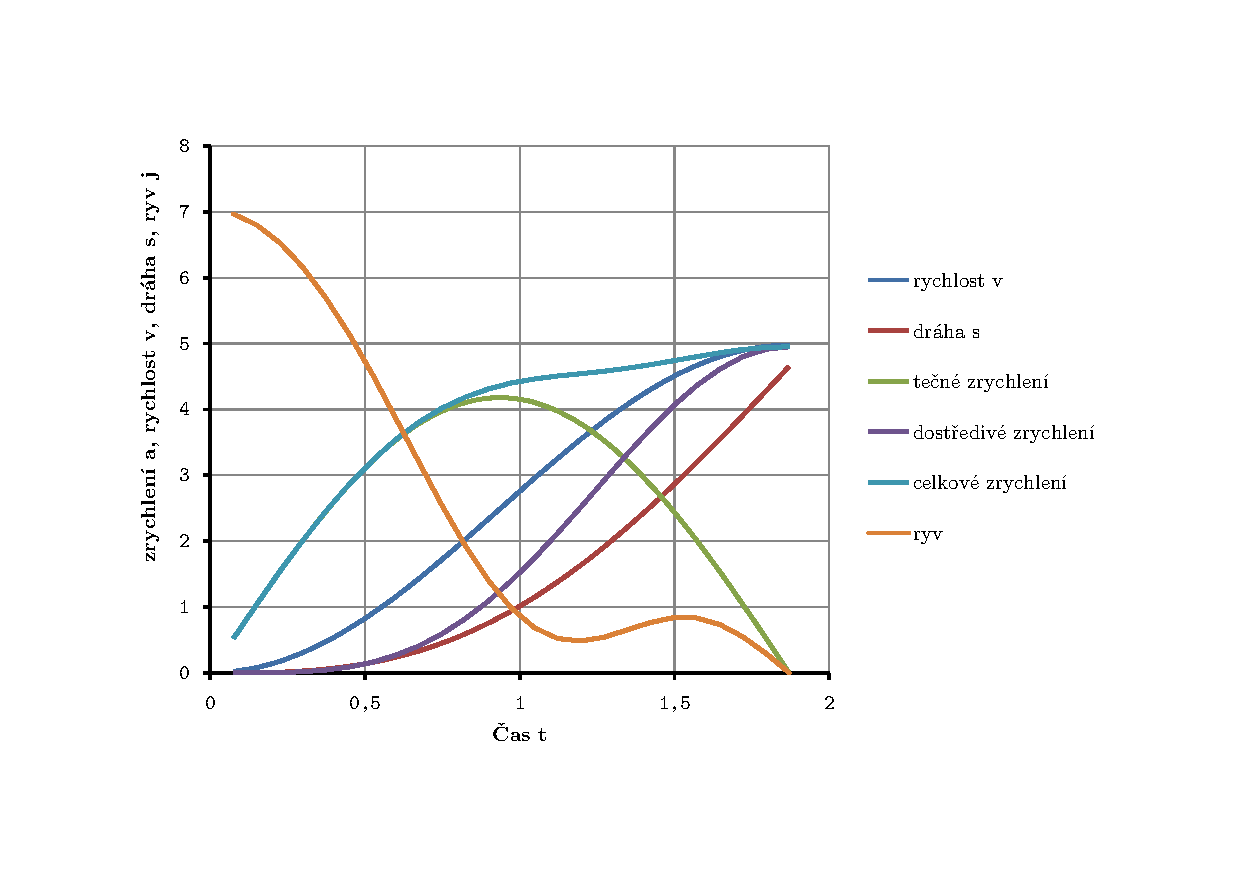
\includegraphics[width=0.9\textwidth]{img/graf_oblouk1.pdf}
		\caption{Graf znázorňující průběh jednotlivých veličin při rozjezdu na oblouku. Maximální hodnota zrychlení se nachází v čase $t=T$.}\label{graf:oblprubeh1}	
	\end{figure}
	\begin{figure}[H]
		\centering
		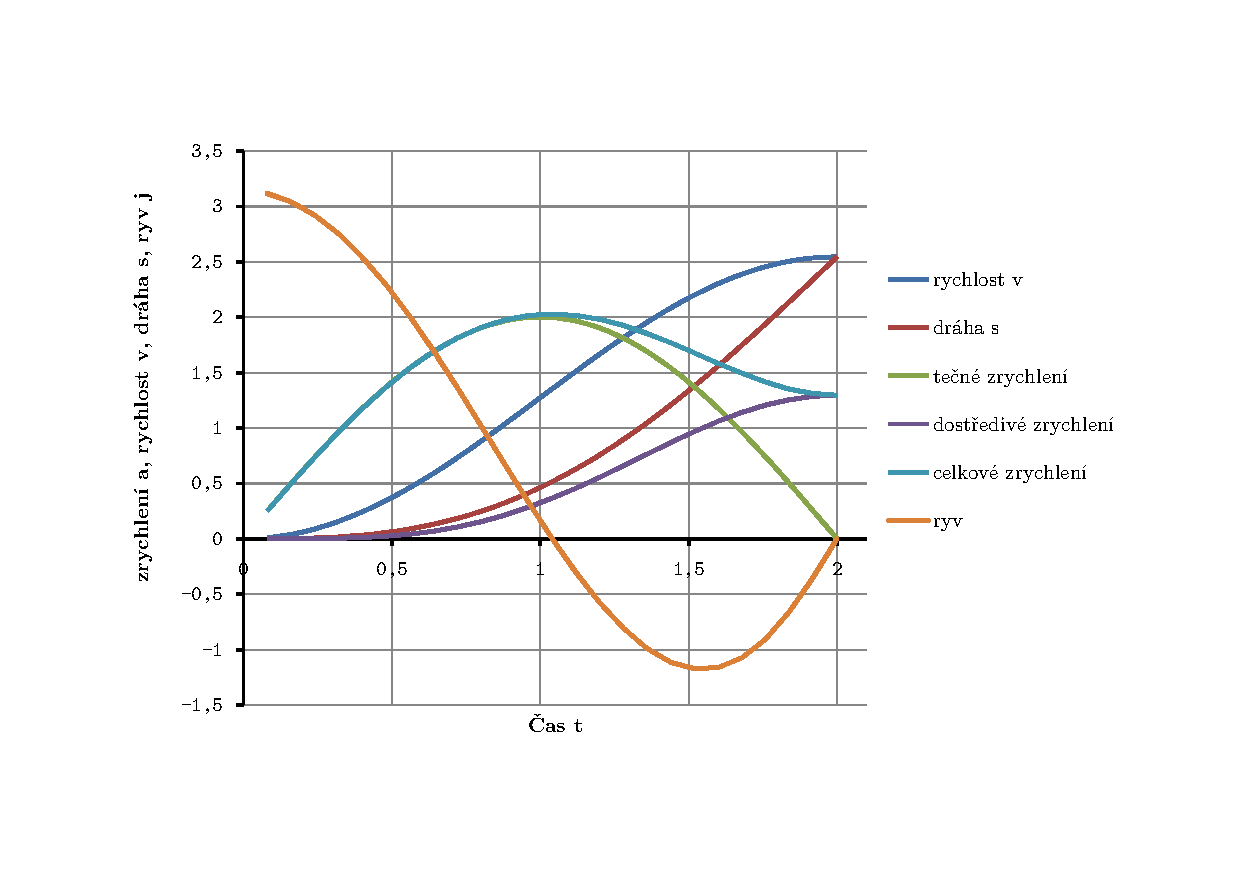
\includegraphics[width=0.9\textwidth]{img/graf_oblouk2.pdf}
		\caption{Graf znázorňující průběh jednotlivých veličin při rozjezdu na oblouku. Maximální hodnota zrychlení se nachází přibližně v~čase $t=\frac{T}{2}$.}\label{graf:oblprubeh2}	
	\end{figure}
	
		\subsection{Maximální zrychlení v čase $t=T$}\label{kap:maxT}
		Tato situace nastává, pokud je maximální dosažitelná rychlost $V$ rovna:
		\begin{equation}\label{rov:oblpodm}
			A_k = \frac{V^2}{r} \implies
			V=\sqrt{A_k r}
		\end{equation}
		Zároveň se však jedná i o podmínku -- při pohybu po~oblouku nelze dosáhnout vyšší rychlosti než výše uvedené -- požadované dostředivé zrychlení by bylo větší než zadané maximální zrychlení.
		
		Jelikož zde neznám hodnotu zrychlení $A$, je třeba pohyb limitovat ryvem. Stejně jako v~případě celkového zrychlení $a_k$ daného vztahem \ref{rov:oblzrych}, je i~v příadě vztahu pro ryv $j$ (\ref{rov:oblryv}) nemožné najít obecné řešení pro jeho maximum. Lze však vypozorovat, že maximum ryvu $j$ se nachází buď v~čase $t=0$, anebo se nachází přibližně na intervalu $t=\left\langle 0,68T; 0,78T\right\rangle$ (tyto hodnoty byly experimentálně vypozorovány).
		
		Pro maximum ryvu $j$ v $t=0$, lze použít stejné vztahy jako pro pohyb po~úsečce -- konkrétně vztah \ref{rov:linTJ} pro výpočet doby pohybu $T$ a~pro výpočet $A$ vztah
		\begin{equation}\label{rov:oblA}
			A = \frac{\pi\sqrt{A_k r}}{2T},
		\end{equation}
		který vychází z~vyjádření zychlení \ref{rov:oblzrych} a~dosazení $t=T$.
		
		Pokud se maximum ryvu nachází na intervalu $t=\left\langle 0,68T; 0,78T\right\rangle$, rozhodl jsem se pro zjednodušení celého výpočtu použít hodnotu maxima pro $t=\frac{3T}{4}$, nikoliv průměr krajních hodnot $0,73T$ -- získám elegatnější tvar koeficientů, které vzniknou z~funkcí sinus a~cosinus.
		
		Dosazením $t=\frac{3T}{4}$ do vztahu pro okamžitý ryv $j$ (\ref{rov:oblryv}) dostanu vztah pro maximální ryv $J$. Pokud k~němu přidám základní vztah pro dobu pohybu $T$ (\ref{rov:lincas}), získám tuto soustavu rovnic:
		\begin{eqnarray}
			\label{rov:oblJT}
			\begin{cases}
			J=\frac{A^4T^4\left(7+5\sqrt{2}\right)-A^2\pi^4r^2}{\pi rT\sqrt{2A^2\pi^4r^2+A^4T^4\left(17+12\sqrt{2}\right)}} \\
			T=\frac{\pi(V-v_0)}{2A}\text{ také lze zapsat jako: }T=\frac{\pi(\sqrt{A_k r}-v_0)}{2A}
			\end{cases}
		\end{eqnarray}
		Tato soustava je řešitelná pouze numericky. Na její řešení jsem použil Newtonovu metodu a~přesný postup výpočtu uvádím v kapitole \ref{kap:newton}.
		
		\subsection{Maximální zrychlení v čase $t=\frac{T}{2}$}\label{kap:maxT2}
		
		Tento případ nastává, pokud je požadovaná rychlost
		\begin{equation}
			V<\sqrt{A_k r}.
		\end{equation}
		Nyní pokud dosadím do vyjádření celkového zrychlení (\ref{rov:oblzrych}) $t=\frac{T}{2}$ a~přidám němu vyjádření času (\ref{rov:lincas}) získám soustavu:
		\begin{eqnarray}\label{rov:oblak}
			\begin{cases}
			A_k = \frac{A\sqrt{\pi^4r^2+A^2T^4}}{\pi^2r} \\
			T = \frac{\pi \left(V-o\right)}{2A}
			\end{cases},
		\end{eqnarray}
		jejímž reálným řešením pro $A$ a~$T$ jsou výrazy:
		\begin{eqnarray}\label{rov:oblt2a}
			A = \frac{16A^2r^2-\left(V-v_0\right)^4}{4r} \nonumber \\
			T = \frac{2\pi r \left(V-v_0\right)}{16A^2r^2-\left(V-v_0\right)^4}
		\end{eqnarray}
		Tím je vyřešeno omezení pohybu z pohledu maximálního dosažitelného zrychlení.
		
		Pro omezení ryvu je třeba najít jeho maxima. První maximum se opět nachází v~$t=0$ a~druhé maxímum opět přibližně v~$t=\frac{3T}{4}$ -- tentokrát však se zápornou hodnotou, protože zrychlení zde klesá (jak lze vidět na grafu \ref{graf:oblprubeh2}).
		
		Pokud se maximum nachází v~čase $t=0$, platí opět stejné vztahy, jako v případě pohybu po~úsečce (vztahy \ref{rov:linTJ}).
		
		Pokud se maximum nachází v~$t=\frac{3T}{4}$, platí vztah \ref{rov:oblJT}, avšak s~opačnou výchylkou ryvu, konkrétně tedy:
		\begin{eqnarray}
			\label{rov:oblJT2}
			\begin{cases}
			-J=\frac{A^4T^4\left(7+5\sqrt{2}\right)-A^2\pi^4r^2}{\pi rT\sqrt{2A^2\pi^4r^2+A^4T^4\left(17+12\sqrt{2}\right)}} \nonumber \\
			T=\frac{\pi(V-v_0)}{2A}
			\end{cases}
		\end{eqnarray}
		
		To jsou všechny vztahy nutné k~popisu rychlosti při pohybu po~kruhovém oblouku. Jejich použití ukazuji v~kapitole \ref{kap:rych-obl}.
		
		\subsection{Problém pohybu po~kruhovém oblouku}
		Pohyb po~kruhovém oblouku se v~praxi používá k~obrábění vnějších rohů obrobku (viz kapitola Implementace korekce nástroje \ref{kap:korekce}). Cílem je zrychlit čas obrábění -- oblouk navazuje na přislušné dráhy nástroje tečně, tudíž se běžně projíždí bez brzdění. Zde však nastává ráz -- aby se nástroj pohyboval po~kruhovém oblouku, musí na něj okamžitě začít působit dostředivé zrychlení. Oblouk bez rázu lze projet pouze pokud se těsně před ním zabrzdí na nulovou rychlost a~až teprve na oblouku se stroj začne rozjíždět.
		
		Jedná se však o natolik běžně používaný postup, že jej i můj řídící systém respektuje a~tečně navazující oblouky projíždí bez brzdění i za cenu vzniklého rázu.
	
	\section{Pohyb po~ideální křivce}\label{kap:krivka}
		Jak jsem zmínil v předcházející sekci, nelze kruhový oblouk projet bez rázu. Rozhodl jsem se proto najít křivku podobnou kruhovému oblouku, kterou lze projet bez brzdění za dodržení všech pravidel postulátu. 
		
		Jak vyplývá z postulátu, musím působit zrychlením ze sinovým průběhem. Také je vhodné, aby toto zrychlení neměnilo směr a~nemusel jsem ještě uvažovat nutné normálové zrychlení. Po~vyzkoušení několika variant jsem dospěl k~uspořádání, které ukazuji na obrázku \ref{obrazek:sinusoida}.
		
		Zrychlení v tomto případě působí kolmo na spojnici A a~B. Poté mohu rozložit rychlost pohybu na složky $v_y$ a~$v_x$ (opět ve směru kolmém, respektive rovnoběžném se spojnicí AB). Rychlost $v_x$ nebude ovlivněna zrychlením -- v~tomto směru se tedy stroj bude pohybovat pohybem rovnoměrným přímočarým. Naopak ve směru rychlosti $v_y$ je stroj nejprve plynule zastaven a~poté se rozjíždí. Výslednou opsanou křivkou je sinusoida. Jelikož je tato křivka symetrická, tak rychlost v~bodě A je stejná jako v~bodě B, pouze se změnil směr pohybu.
		
		Pro určení maximálního zrychlení $A$ lze použít vztah pro maximální zrychlení na přímce (\ref{rov:linzrych}) -- zajímá nás totiž pouze změna zrychlení ve směru rychlosti $v_y$. Dobu pohybu určíme z~rychlosti $v_x$ -- stroj musí urazit vzdálenost $\abs{A-B}$ rychlostí $v_x$, tedy:
		\begin{equation}
			T = \frac{\abs{A-B}}{v_x}
		\end{equation}
		Změna rychlosti, výraz $V-v_0$ v~původním vztahu, je rovnen $2v_y$, jelikož rychlost $v_y$ se změní na opačnou. Celkově tedy platí:
		\begin{equation}
			A = \frac{\pi v_xv_y}{\abs{A-B}}
		\end{equation}
		
		\begin{figure}[h]
			\centering
			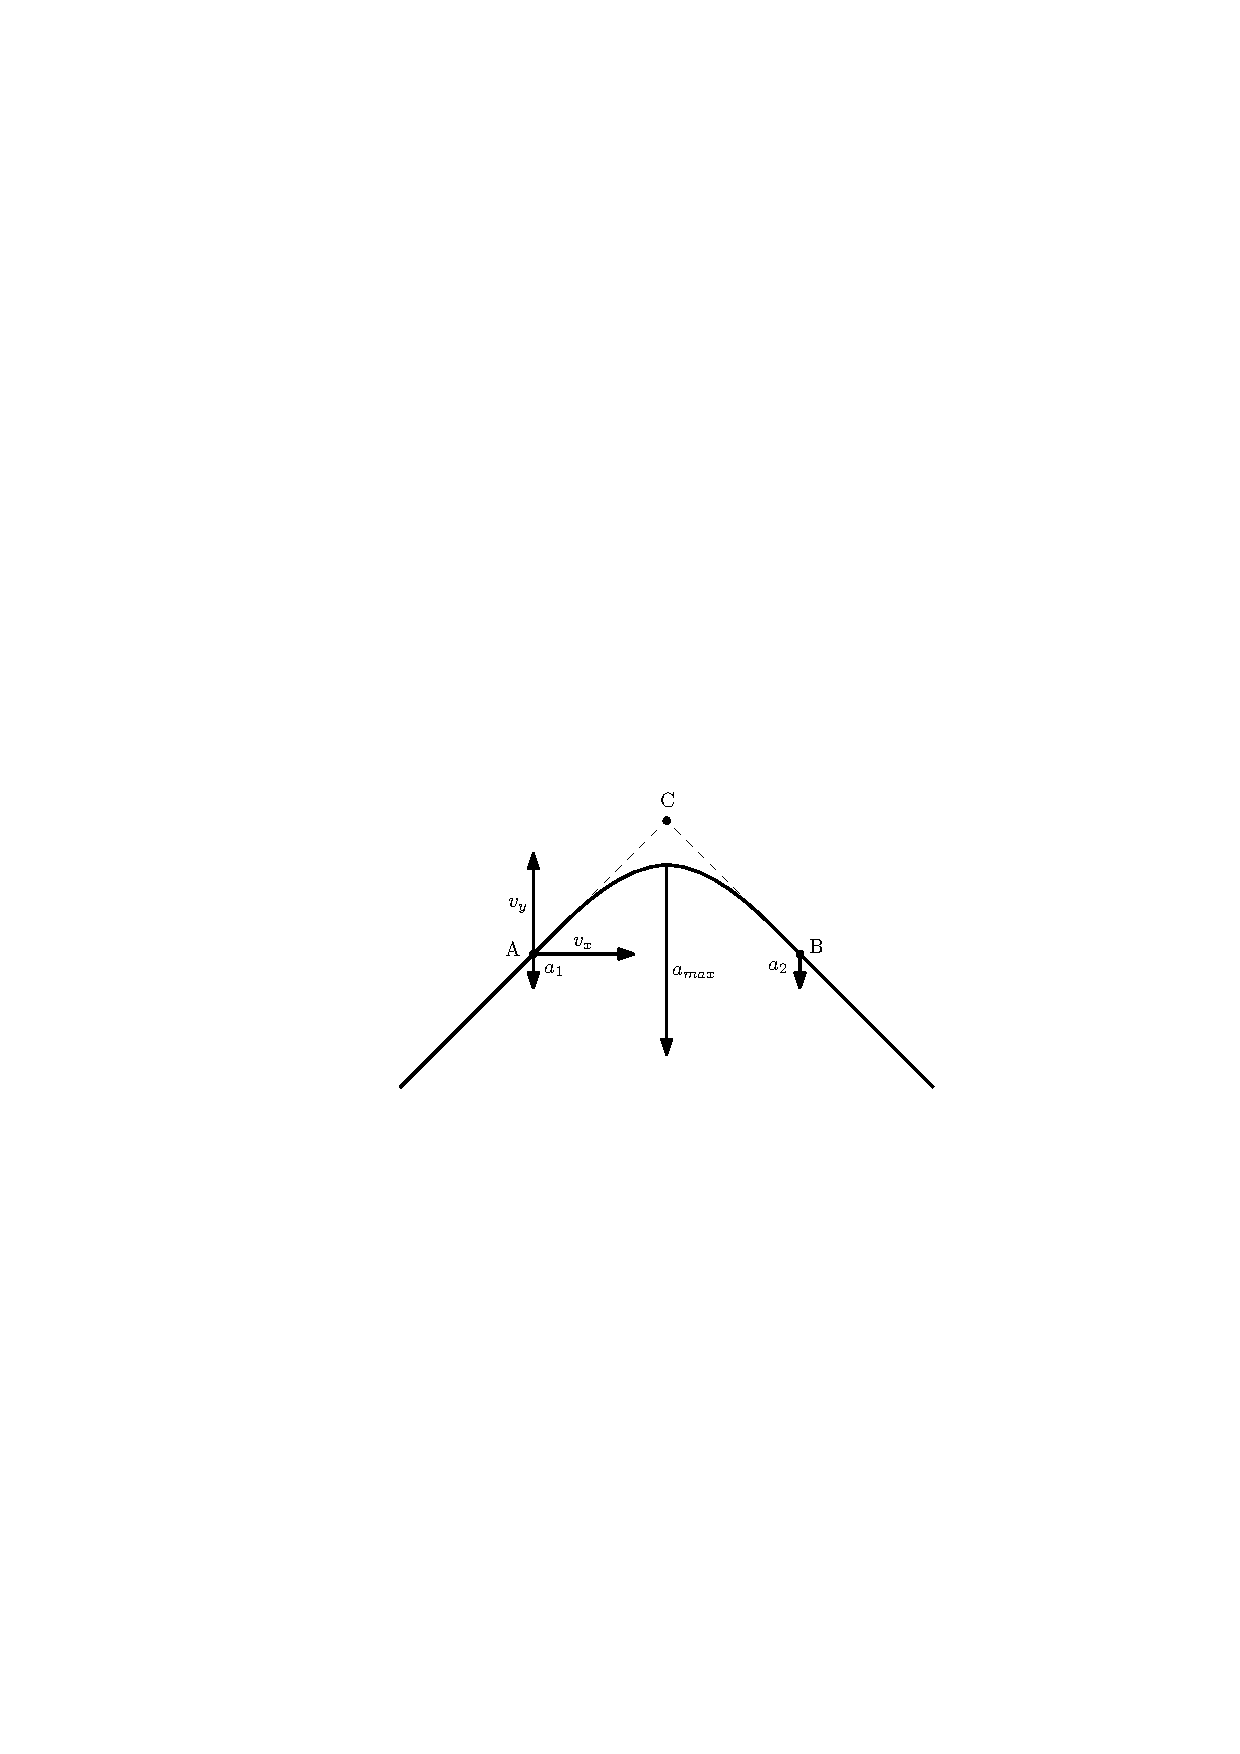
\includegraphics[width=0.6\textwidth]{img/sinusoida.pdf}
			\caption{Obrázek znázorňující \uv{ideální křivku} -- sinusoidu. Zrychleními $a_1$, $a_{max}$ a~$a_2$ je zde naznačen sinusový průběh zrychlení.} \label{obrazek:sinusoida}
		\end{figure}
		
		Tato křivka je však nevhodná pro obrábění -- upřednostňuje totiž dynamiku pohybu před přesností obrábění. Původně jsem zamýšlel použít tuto křivku k~\uv{zakulacení} rohů pohybu rychloposuvem, kde by nepřesnost nemusela vadit. Avšak nemůžu garantovat, že i při rychloposuvu by zůstal dostatek místa pro zkreslení trajektorie tak, aby stroj nenaboural do obrobku, jelikož CAM program toto zkreslení nemůže předpokládat -- ač bývá zvykem při rychloposuvu nechávat co nejvíce místa mezi strojem a~obrobkem. Proto jsem od myšlenky implementovat tuto křivku upustil a~ani jsem ji nějak dále nerozvíjel -- proto jsem ji nezkoumal z~hlediska omezení ryvu a~nalezení mezních rychlostí.